\HeadingLevelB{SGX Enclave Launch Control}
\label{sec:sgx_launch_control}

The SGX design includes a launch control process, which introduces an
unnecessary approval step that is required before running most enclaves on a
computer. The approval decision is made by the \textit{Launch Enclave} (LE),
which is an enclave issued by Intel that gets to approve every other enclave
before it is initialized by \textit{EINIT}~(\S~\ref{sec:sgx_einit_overview}).
The officially documented information about this approval process is discussed
in \S~\ref{sec:sgx_launch_enclave}.

% Enclave License
%   US 8,972,746 B2 - 34:6-23
% Licenses are evaluated into Permits (which became EINITTTOKEN)
%   US 8,972,746 B2 - 34:24-29, 35:27-59
% EINIT requires a Permit to launch a production enclave
%   US 8,972,746 B2 - 35:60-67, 36:1-3, 36:47-52, 38:4-65
% License Enclave creates Permit
%   US 8,972,746 B2 - 36:40-46, 37:50-67, 38:1-3
% EMKPERMIT seems to have gotten merged into EINIT
%   US 8,972,746 B2 - 36:53-67, 37:1-7, 37:24-49
% License became SIGSTRUCT
%   US 8,972,746 B2 - 37:8-23

The SGX patents~\cite{intel2013patent1, intel2013patent2} disclose in no
uncertain terms that the Launch Enclave was introduced to ensure that each
enclave's author has a business relationship with Intel, and implements a
software licensing system. \S~\ref{sec:sgx_licensing} briefly discusses the
implications, should this turn out to be true.

The remainder of the section argues that the Launch Enclave should be removed
from the SGX design. \S~\ref{sec:sgx_provisioning_privacy} explains that the
LE is not required to enforce the computer owner's launch control policy, and
concludes that the LE is only meaningful if it enforces a policy that is
detrimental to the computer owner. \S~\ref{sec:sgx_enclaves_vs_system} debunks
the myth that an enclave can host malware, which is likely to be used to
justify the LE. \S~\ref{sec:sgx_enclaves_vs_av} argues that Anti-Virus (AV)
software is not fundamentally incompatible with enclaves, further disproving
the theory that Intel needs to actively police the software that runs inside
enclaves.


\HeadingLevelC{Enclave Attributes Access Control}
\label{sec:sgx_launch_enclave}

% ATTRIBUTES: SDM S 38.7.1

The SGX design requires that all enclaves be vetted by a Launch Enclave~(LE),
which is only briefly mentioned in Intel's official documentation. Neither its
behavior nor its interface with the system software is specified. We speculate
that Intel has not been forthcoming about the LE because of its role in
enforcing software licensing, which will be discussed in
\S~\ref{sec:sgx_licensing}. This section abstracts away the licensing aspect
and assumes that the LE enforces a black-box Launch Control Policy.

The LE approves an enclave by issuing an \textit{EINIT Token}~(EINITTOKEN),
using the process illustrated in Figure~\ref{fig:sgx_einittoken}. The
EINITTOKEN structure contains the approved enclave's
measurement-based~(\S~\ref{sec:sgx_measurement}) and
certificate-based~(\S~\ref{sec:sgx_certificate_identity}) identities, just like
a local attestation REPORT~(\S~\ref{sec:sgx_ereport}). This token is inspected
by \texttt{EINIT}~(\S~\ref{sec:sgx_einit_overview}), which refuses to
initialize enclaves with incorrect tokens.

\begin{figure}[hbt!]
  \centering
  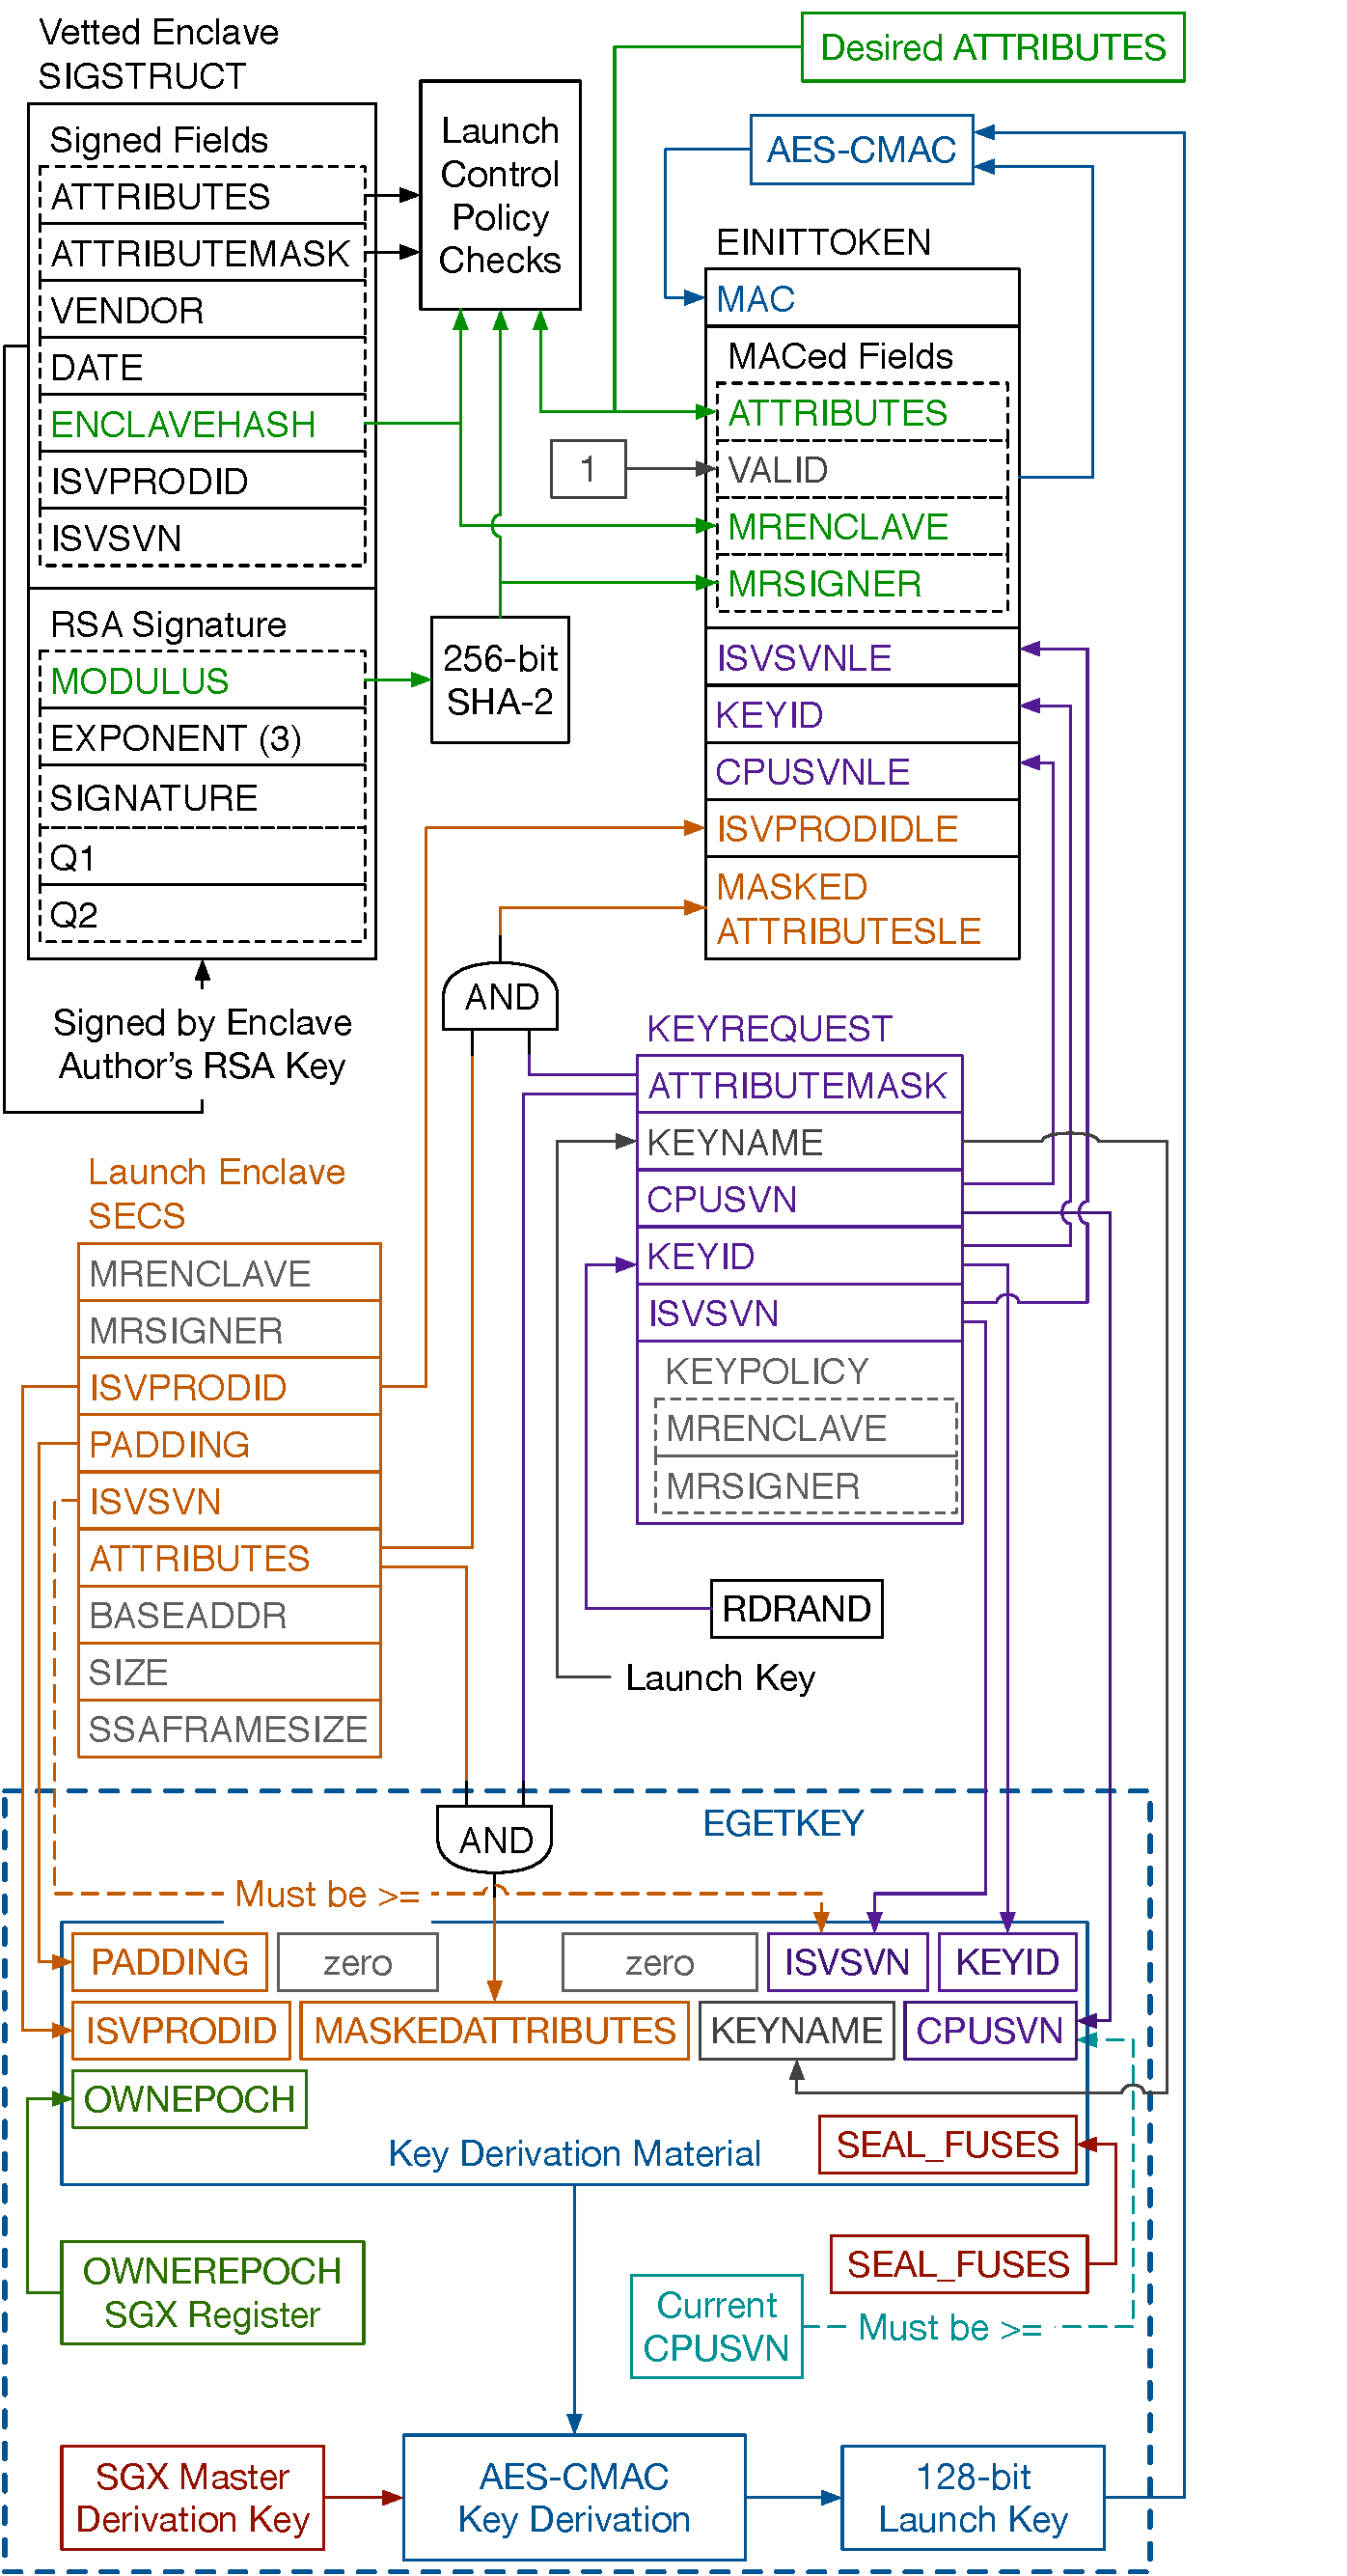
\includegraphics[width=95mm]{figures/sgx_einittoken.pdf}
  \caption{
    The SGX Launch Enclave computes the EINITTOKEN.
  }
  \label{fig:sgx_einittoken}
\end{figure}

% EINIT Token Structure (EINITTOKEN): SDM S 38.14

While an EINIT token is handled by untrusted system software, its integrity is
protected by a MAC tag~(\S~\ref{sec:integrity_crypto}) that is computed using a
\textit{Launch Key} obtained from \texttt{EGETKEY}. The \texttt{EINIT}
implementation follows the same key derivation process as \texttt{EGETKEY} to
convince itself that the EINITTOKEN provided to it was indeed generated by an
LE that had access to the Launch Key.

The SDM does not document the MAC algorithm used to confer integrity guarantees
to the EINITTOKEN structure. However, the \texttt{EINIT} pseudocode verifies
the token's MAC tag using the same function that the \textit{EREPORT}
pseudocode uses to create the REPORT structure's MAC tag. It follows that the
reasoning in \S~\ref{sec:sgx_ereport} can be reused to conclude that EINITTOKEN
structures are MACed using AES-CMAC with 128-bit keys.

% EGETKEY: SDM S 41.4.1
% Key Derivation: SDM Table 41-43

The \texttt{EGETKEY} instruction only derives the Launch Key for enclaves that
have the LAUNCHKEY attribute set to true. The Launch Key is derived using the
same process as the Seal Key~(\S~\ref{sec:sgx_egetkey}). The derivation material
includes the current enclave's versioning information (ISVPRODID and ISVSVN)
but it does not include the main fields that convey an enclave's identity,
which are MRSIGNER and MRENCLAVE. The rest of the derivation material follows
the same rules as the material used for Seal Keys.

The EINITTTOKEN structure contains the identities of the approved enclave
(MRENCLAVE and MRSIGNER) and the approved enclave attributes (ATTRIBUTES). The
token also includes the information used for the Launch Key derivation,
which includes the LE's Product ID (ISVPRODIDLE), SVN (ISVSVNLE), and the
bitwise AND between the LE's ATTRIBUTES and the ATTRIBUTEMASK used in the
KEYREQUEST (MASKEDATTRIBUTESLE).

The EINITTOKEN information used to derive the Launch Key can also be used
by \texttt{EINIT} for damage control, e.g. to reject tokens issued by Launch
Enclaves with known security vulnerabilities. The reference pseudocode supplied
in the SDM states that \texttt{EINIT} checks the DEBUG bit in the
MASKEDATTRIBUTESLE field, and will not initialize a production enclave using
a token issued by a debugging LE. It is worth noting that MASKEDATTRIBUTESLE is
guaranteed to include the LE's DEBUG attribute, because \texttt{EGETKEY} forces
the DEBUG attribute's bit in the attributes mask to 1
(\S~\ref{sec:sgx_egetkey}).

The check described above make it safe for Intel to supply SGX enclave
developers with a debugging LE that has its DEBUG attribute set, and performs
minimal or no security checks before issuing an EINITTOKEN. The DEBUG attribute
disables SGX's integrity protection, so the only purpose of the security checks
performed in the debug LE would be to help enclave development by mimicking its
production counterpart. The debugging LE can only be used to launch any enclave
with the DEBUG attribute set, so it does not undermining Intel's ability to
enforce a Launch Control Policy on production enclaves.

% EINIT: SDM S 41.3
% EINITTOKENKEY is bit 5, INTEL_ONLY_MASK is 0x20

The enclave attributes access control system described above relies on the LE
to reject initialization requests that set privileged attributes such as
PROVISIONKEY on unauthorized enclaves. However, the LE cannot vet itself, as
there will be no LE available when the LE itself needs to be initialized.
Therefore, the Launch Key access restrictions are implemented in hardware.

\texttt{EINIT} accepts an EINITTOKEN whose VALID bit is set to zero, if
the enclave's MRSIGNER~(\S~\ref{sec:sgx_mrsigner}) equals a hard-coded value
that corresponds to an Intel public key. For all other enclave authors, an
invalid EINIT token causes \texttt{EINIT} to reject the enclave and produce an
error code.

This exemption to the token verification policy provides a way to bootstrap the
enclave attributes access control system, namely using a zeroed out EINITTOKEN
to initialize the Launch Enclave. At the same time, the cryptographic
primitives behind the MRSIGNER check guarantee that only Intel-provided
enclaves will be able to bypass the attribute checks. This does not change
SGX's security properties because Intel is already a trusted party, as it is
responsible for generating the Provisioning Keys and Attestation Keys used by
software attestation~(\S~\ref{sec:sgx_quoting_enclave}).

Curiously, the \texttt{EINIT} pseudocode in the SDM states that the instruction
enforces an additional restriction, which is that all enclaves with the
LAUNCHKEY attribute must have its certificate issued by the same Intel public
key that is used to bypass the EINITTTOKEN checks. This restriction appears to
be redundant, as the same restriction could be enforced in the Launch Enclave.


\HeadingLevelC{Licensing}
\label{sec:sgx_licensing}

The SGX patents~\cite{intel2013patent1, intel2013patent2} disclose that
\texttt{EINIT} Tokens and the Launch Enclave~(\S~\ref{sec:sgx_launch_enclave})
were introduced to verify that the SIGSTRUCT certificates associated with
production enclaves are issued by enclave authors who have a business
relationship with Intel. In other words, the Launch Enclave is intended to be
\textbf{an enclave licensing mechanism that allows Intel to force itself as an
intermediary in the distribution of all enclave software}.

The SGX patents are likely to represent an early version of the SGX design, due
to the lengthy timelines associated with patent application approval.
In light of this consideration, we cannot make any claims about Intel's current
plans. However, given that we know for sure that Intel considered enclave
licensing at some point, we briefly discuss the implications of implementing
such a licensing plan.

Intel has a near-monopoly on desktop and server-class processors, and being
able to decide which software vendors are allowed to use SGX can effectively
put Intel in a position to decide winners and losers in many software markets.

Assuming SGX reaches widespread adoption, this issue is the software security
equivalent to the Net Neutrality debates that have pitted the software industry
against telecommunication giants. Given that virtually all competent software
development companies have argued that losing Net Neutrality will stifle
innovation, it is fairly safe to assume that Intel's ability to regulate access
to SGX will also stifle innovation.

Furthermore, from a historical perspective, the enclave licensing scheme
described in the SGX patents is very similar to Verified Boot, which was
briefly discussed in \S~\ref{sec:sgx_related_tpm}. Verified Boot has mostly
received negative reactions from software developers, so it is likely that an
enclave licensing scheme would meet the same fate, should the developer
community become aware of it.


\HeadingLevelC{System Software Can Enforce a Launch Policy}
\label{sec:sgx_provisioning_privacy}

\S~\ref{sec:sgx_enclave_lifecycle} explains that the SGX instructions used to
load and initialize enclaves (\texttt{ECREATE}, \texttt{EADD}, \texttt{EINIT})
can only be issued by privileged system software, because they manage the EPC,
which is a system resource.

A consequence on the restriction that only privileged software can issue
\texttt{ECREATE} and \texttt{EADD} instructions is that the system software is
able to track all the public contents that is loaded into each enclave. The
privilege requirements of \texttt{EINIT} mean that the system software can also
examine each enclave's SIGSTRUCT. It follows that the system software has
access to a superset of the information that the Launch Enclave might use.

Furtheremore, \texttt{EINIT}'s privileged instruction status means that the
system software can perform its own policy checks before allowing application
software to initialize an enclave. So, the system software can enforce a Launch
Control Policy set by the computer's owner. For example, an IaaS cloud service
provider may use its hypervisor to implement a Launch Control Policy that
limits what enclaves its customers are allowed to execute.

Given that the system software has access to a superset of the information that
the Launch Enclave might use, it is easy to see that the set of policies that
can be enforced by system software is a superset of the policies that can be
supported by an LE. Therefore, the only rational explanation for the existence
of the LE is that it was designed to implement a Launch Control Policy that is
not beneficial to the computer owner.

As an illustration of this argument, we consider the case of restricting access
to \texttt{EGETKEY}'s Provisioning keys~(\S~\ref{sec:sgx_quoting_enclave}).
The derivation material for Provisioning keys does not include OWNEREPOCH, so
malicious enclaves can potentially use these keys to track a CPU chip package
as it exchanges owners. For this reason, the SGX design includes a simple
access control mechanism that can be used by system software to limiting
enclave access to Provisioning keys. \texttt{EGETKEY} refuses to derive
Provisioning keys for enclaves whose PROVISIONKEY attribute is not set to true.

It follows that a reasonable Launch Control Policy would only allow the
PROVISIONKEY attribute to be set for the enclaves that implement software
attestation, such as Intel's Provisioning Enclave and Quoting Enclave. This
policy can easily be implemented by system software, given its exclusive access
to the \texttt{EINIT} instruction.

The only concern with the approach outlined above is that a malicious system
software might abuse the PROVISIONKEY attribute to generate a unique identifier
for the hardware that it runs on, similar to the much maligned Intel Processor
Serial Number~\cite{intel1999psn}. We dismiss this concern by pointing out that
system software has access to many unique identifiers, such as the
Media Access Control~(MAC) address of the Ethernet adapter integrated into the
motherboard's chipset~(\S~\ref{sec:motherboard}).


\HeadingLevelC{Enclaves Cannot Damage the Host Computer}
\label{sec:sgx_enclaves_vs_system}
% NOTE: This is a slightly edited answer to a question we received.

SGX enclaves execute at the lowest privilege level (user mode / ring 3), so
they are subject to the same security checks as their host application. For
example, modern operating systems set up the I/O maps~(\S~\ref{sec:segments})
to prevent application software from directly accessing the I/O address
space~(\S~\ref{sec:address_spaces}), and use the supervisor (S) page table
attribute~(\S~\ref{sec:page_table_attributes}) to deny application software
direct access to memory-mapped devices~(\S~\ref{sec:address_spaces}) and to the
DRAM that stores the system software. Enclave software is subject to I/O
privilege checks and address translation checks, so a malicious enclave cannot
directly interact with the computer's devices, and cannot tamper the system
software.

It follows that software running in an enclave has the same means to compromise
the system software as its host application, which come down to exploiting a
security vulnerability. The same solutions used to mitigate vulnerabilities
exploited by application software (e.g.,
\texttt{seccomp/bpf}~\cite{kim2013seccompbpf}) apply to enclaves.

The only remaining concern is that an enclave can perform a denial of service
(DoS) attack against the system software. The rest of this section addresses
the concern.

The SGX design provides system software the tools it needs to protect itself
from enclaves that engage in CPU hogging and DRAM hogging. As enclaves cannot
perform I/O directly, these are the only two classes of DoS attacks available
to them.

An enclave that attempts to hog an LP assigned to it can be preempted by the
system software via an Inter-Processor Interrupt~(IPI,~\S~\ref{sec:interrupts})
issued from another processor. This method is available as long as the system
software reserves at least one LP for non-enclave computation.

Furthermore, most OS kernels use tick schedulers, which use a real-time clock
(RTC) configured to issue periodical interrupts (ticks) to all cores. The RTC
interrupt handler invokes the kernel's scheduler, which chooses the thread that
will get to use the logical processor until the next RTC interrupt is received.
Therefore, kernels that use tick schedulers always have the opportunity to
de-schedule enclave threads, and don't need to rely on the ability to send
IPIs.

In SGX, the system software can always evict an enclave's EPC pages to non-EPC
memory, and then to disk. The system software can also outright deallocate an
enclave's EPC pages, though this will probably cause the enclave code to
encounter page faults that cannot be resolved. The only catch is that the EPC
pages that hold metadata for running enclave threads cannot be evicted or
removed. However, this can easily be resolved, as the system software can
always preempt enclave threads, using one of the methods described above.

% TODO(pwnall): Move the following paragraphs into Sanctum.
%Sanctum gives the system software less control over the DRAM regions allocated
%to enclaves, in order to hide the enclaves' memory access patterns.
%Specifically, the system software cannot reclaim a DRAM region from an enclave
%without the enclave's cooperation. However, the system software can always
%completely terminate an enclave and reclaim all its memory.
%
%Sanctum's enclaves can only be terminated when all their threads are stopped.
%Therefore, when the system software decides that an enclave is hogging CPU or
%DRAM, it can preempt all the enclave's threads, using the methods described
%above, and then terminate the enclave.


\HeadingLevelC{Interaction with Anti-Virus Software}
\label{sec:sgx_enclaves_vs_av}
% NOTE: This is a slightly edited answer to a question we received.

Today's anti-virus (AV) systems are glorified pattern matchers. AV software
simply scans all the executable files on the system and the memory of running
processes, looking for bit patterns that are thought to only occur in malicious
software. These patterns are somewhat pompously called ``virus signatures".

SGX (and TXT, to some extent) provides a method for executing code in an
isolated container that we refer to as an enclave. Enclaves are isolated from
all the other software on the computer, including any AV software that might be
installed.

The isolation afforded by SGX opens up the possibility for bad actors to
structure their attacks as a generic loader that would end up executing a
malicious payload without tripping the AV's pattern matcher.  More
specifically, the attack would create an enclave and initialize it with a
generic loader that looks innocent to an AV. The loader inside the enclave
would obtain an encrypted malicious payload, and would undergo software
attestation with an Internet server to obtain the payload's encryption key. The
loader would then decrypt the malicious payload and execute it inside the
enclave.

In the scheme suggested here, the malicious payload only exists in a decrypted
form inside an enclave's memory, which cannot be accessed by the AV. Therefore,
the AV's pattern matcher will not trip.

This issue does not have a solution that maintains the status-quo for the AV
vendors. The attack described above would be called a protection scheme if the
payload would be a proprietary image processing algorithm, or a DRM scheme.

On a brighter note, enclaves do not bring the complete extinction of AV, they
merely require a change in approach. Enclave code always executes at the lowest
privilege mode (ring 3 / user mode), so it cannot perform any I/O without
invoking the services of system software. For all intents and purposes, this
effectively means that enclave software cannot perform any malicious action
without the complicity of system software. Therefore, enclaves can be policed
effectively by intelligent AV software that records and filters the I/O
performed by software, and detects malicious software according to the actions
that it performs, rather than according to bit patterns in its code.

Furthermore, SGX's enclave loading model allows the possibility of performing
static analysis on the enclave's software. For simplicity, assume the existence
of a standardized static analysis framework.  The initial enclave contents is
not encrypted, so the system software can easily perform static analysis on it.
Dynamically loaded code or Just-In-Time code generation (JIT) can be handled by
requiring that all enclaves that use these techniques embed the static analysis
framework and use it to analyze any dynamically loaded code before it is
executed. The system software can use static verification to ensure that
enclaves follow these rules, and refuse to initialize any enclaves that fail
verification.

In conclusion, enclaves in and of themselves don't introduce new attack vectors
for malware. However, the enclave isolation mechanism is fundamentally
incompatible with the approach employed by today's AV solutions. Fortunately,
it is possible (though non-trivial) to develop more intelligent AV software for
enclave software.
